% Options for packages loaded elsewhere
\PassOptionsToPackage{unicode}{hyperref}
\PassOptionsToPackage{hyphens}{url}
\PassOptionsToPackage{dvipsnames,svgnames,x11names}{xcolor}
%
\documentclass[
  11pt,
]{article}

\usepackage{amsmath,amssymb}
\usepackage{iftex}
\ifPDFTeX
  \usepackage[T1]{fontenc}
  \usepackage[utf8]{inputenc}
  \usepackage{textcomp} % provide euro and other symbols
\else % if luatex or xetex
  \usepackage{unicode-math}
  \defaultfontfeatures{Scale=MatchLowercase}
  \defaultfontfeatures[\rmfamily]{Ligatures=TeX,Scale=1}
\fi
\usepackage{lmodern}
\ifPDFTeX\else  
    % xetex/luatex font selection
\fi
% Use upquote if available, for straight quotes in verbatim environments
\IfFileExists{upquote.sty}{\usepackage{upquote}}{}
\IfFileExists{microtype.sty}{% use microtype if available
  \usepackage[]{microtype}
  \UseMicrotypeSet[protrusion]{basicmath} % disable protrusion for tt fonts
}{}
\makeatletter
\@ifundefined{KOMAClassName}{% if non-KOMA class
  \IfFileExists{parskip.sty}{%
    \usepackage{parskip}
  }{% else
    \setlength{\parindent}{0pt}
    \setlength{\parskip}{6pt plus 2pt minus 1pt}}
}{% if KOMA class
  \KOMAoptions{parskip=half}}
\makeatother
\usepackage{xcolor}
\usepackage[lmargin=1in,rmargin=1in,tmargin=1in,bmargin=1in]{geometry}
\setlength{\emergencystretch}{3em} % prevent overfull lines
\setcounter{secnumdepth}{3}
% Make \paragraph and \subparagraph free-standing
\ifx\paragraph\undefined\else
  \let\oldparagraph\paragraph
  \renewcommand{\paragraph}[1]{\oldparagraph{#1}\mbox{}}
\fi
\ifx\subparagraph\undefined\else
  \let\oldsubparagraph\subparagraph
  \renewcommand{\subparagraph}[1]{\oldsubparagraph{#1}\mbox{}}
\fi


\providecommand{\tightlist}{%
  \setlength{\itemsep}{0pt}\setlength{\parskip}{0pt}}\usepackage{longtable,booktabs,array}
\usepackage{calc} % for calculating minipage widths
% Correct order of tables after \paragraph or \subparagraph
\usepackage{etoolbox}
\makeatletter
\patchcmd\longtable{\par}{\if@noskipsec\mbox{}\fi\par}{}{}
\makeatother
% Allow footnotes in longtable head/foot
\IfFileExists{footnotehyper.sty}{\usepackage{footnotehyper}}{\usepackage{footnote}}
\makesavenoteenv{longtable}
\usepackage{graphicx}
\makeatletter
\def\maxwidth{\ifdim\Gin@nat@width>\linewidth\linewidth\else\Gin@nat@width\fi}
\def\maxheight{\ifdim\Gin@nat@height>\textheight\textheight\else\Gin@nat@height\fi}
\makeatother
% Scale images if necessary, so that they will not overflow the page
% margins by default, and it is still possible to overwrite the defaults
% using explicit options in \includegraphics[width, height, ...]{}
\setkeys{Gin}{width=\maxwidth,height=\maxheight,keepaspectratio}
% Set default figure placement to htbp
\makeatletter
\def\fps@figure{htbp}
\makeatother
% definitions for citeproc citations
\NewDocumentCommand\citeproctext{}{}
\NewDocumentCommand\citeproc{mm}{%
  \begingroup\def\citeproctext{#2}\cite{#1}\endgroup}
\makeatletter
 % allow citations to break across lines
 \let\@cite@ofmt\@firstofone
 % avoid brackets around text for \cite:
 \def\@biblabel#1{}
 \def\@cite#1#2{{#1\if@tempswa , #2\fi}}
\makeatother
\newlength{\cslhangindent}
\setlength{\cslhangindent}{1.5em}
\newlength{\csllabelwidth}
\setlength{\csllabelwidth}{3em}
\newenvironment{CSLReferences}[2] % #1 hanging-indent, #2 entry-spacing
 {\begin{list}{}{%
  \setlength{\itemindent}{0pt}
  \setlength{\leftmargin}{0pt}
  \setlength{\parsep}{0pt}
  % turn on hanging indent if param 1 is 1
  \ifodd #1
   \setlength{\leftmargin}{\cslhangindent}
   \setlength{\itemindent}{-1\cslhangindent}
  \fi
  % set entry spacing
  \setlength{\itemsep}{#2\baselineskip}}}
 {\end{list}}
\usepackage{calc}
\newcommand{\CSLBlock}[1]{\hfill\break\parbox[t]{\linewidth}{\strut\ignorespaces#1\strut}}
\newcommand{\CSLLeftMargin}[1]{\parbox[t]{\csllabelwidth}{\strut#1\strut}}
\newcommand{\CSLRightInline}[1]{\parbox[t]{\linewidth - \csllabelwidth}{\strut#1\strut}}
\newcommand{\CSLIndent}[1]{\hspace{\cslhangindent}#1}

\makeatletter
\@ifpackageloaded{caption}{}{\usepackage{caption}}
\AtBeginDocument{%
\ifdefined\contentsname
  \renewcommand*\contentsname{Table of contents}
\else
  \newcommand\contentsname{Table of contents}
\fi
\ifdefined\listfigurename
  \renewcommand*\listfigurename{List of Figures}
\else
  \newcommand\listfigurename{List of Figures}
\fi
\ifdefined\listtablename
  \renewcommand*\listtablename{List of Tables}
\else
  \newcommand\listtablename{List of Tables}
\fi
\ifdefined\figurename
  \renewcommand*\figurename{Figure}
\else
  \newcommand\figurename{Figure}
\fi
\ifdefined\tablename
  \renewcommand*\tablename{Table}
\else
  \newcommand\tablename{Table}
\fi
}
\@ifpackageloaded{float}{}{\usepackage{float}}
\floatstyle{ruled}
\@ifundefined{c@chapter}{\newfloat{codelisting}{h}{lop}}{\newfloat{codelisting}{h}{lop}[chapter]}
\floatname{codelisting}{Listing}
\newcommand*\listoflistings{\listof{codelisting}{List of Listings}}
\makeatother
\makeatletter
\makeatother
\makeatletter
\@ifpackageloaded{caption}{}{\usepackage{caption}}
\@ifpackageloaded{subcaption}{}{\usepackage{subcaption}}
\makeatother
\ifLuaTeX
  \usepackage{selnolig}  % disable illegal ligatures
\fi
\usepackage{bookmark}

\IfFileExists{xurl.sty}{\usepackage{xurl}}{} % add URL line breaks if available
\urlstyle{same} % disable monospaced font for URLs
\hypersetup{
  pdftitle={Redistribution and Time Poverty: Balancing Responsibilities in Couple Households},
  pdfauthor={Fernando Rios-Avila; Aashima Sinha},
  pdfkeywords={Time Poverty, Income Poverty, Redistribution, household
production, care work, gender equality, LIMTIP},
  colorlinks=true,
  linkcolor={blue},
  filecolor={Maroon},
  citecolor={Blue},
  urlcolor={Blue},
  pdfcreator={LaTeX via pandoc}}


\usepackage{datetime}
\usepackage{booktabs}
\usepackage{chngcntr}
\usepackage{apptools}
\usepackage{lipsum}
\usepackage{booktabs}
\usepackage{multirow}
\usepackage{makecell}
\AtAppendix{\counterwithin{table}{section}}
\AtAppendix{\counterwithin{figure}{section}}

\title{Redistribution and Time Poverty: Balancing Responsibilities in
Couple Households}
\author{
Fernando Rios-Avila\\
Levy Economics Institute\\
\\
\and 
Aashima Sinha\\
Levy Economics Institute\\
\\
}
\date{2024-12-03}
\begin{document}


\def\spacingset#1{\renewcommand{\baselinestretch}%
{#1}\small\normalsize} \spacingset{1}

%Ipsum lorem

\maketitle
\begin{abstract}
This policy brief examines how redistributing household production
responsibilities could reduce time poverty among married U.S. couples.
Using the Levy Institute Measure of Time and Income Poverty (LIMTIP), we
analyze three redistriution scenarios based on equality, equity, and
opportunity cost principles, over the period 2015-19. Our findings show
that redistribution could effectively reduce time poverty for married
couples, particularly in households where time surplus exceeds deficits;
with the equity-based approach proving most successful. The reduction in
time poverty comes with greater gender-equitable sharing of housework
between couples. Additionally, redistribution can potentially lift
households out of poverty and reduce the share of hidden poor; thus
providing insights into improving the scope of poverty alleviation
programs. The effectiveness of redistribution varies across household
types and structures, suggesting targeted approaches may work better
than universal solutions.
\end{abstract}
 
\vspace{.2in}

\textbf{\textit{Keyword: }}Time Poverty, Income Poverty, Redistribution,
household production, care work, gender equality, LIMTIP


\thispagestyle{empty}
\clearpage\pagenumbering{arabic}
\newpage
\spacingset{1.2} % DON'T change the spacing!
\section{Introduction}\label{introduction}

Redistribution of household production, which includes unpaid caregiving
and domestic chores, has been identified as an important tool to achieve
gender equality. The United Nations Sustainable Development Goal 5,
Target 5.4, has incorporated the recognition, reduction, and
redistribution of unpaid work strategy, popularly known as the 3R
strategy. This is a testament to decades of activism and advocacy
emphasizing that gender inequality on this front cannot be simply
justified as a ``private family matter'', but rather be considered a
matter of public policy. Redistribution can take place from households
to the public and/or private spheres, as well as among household
members. Evidence shows that it is disproportionately undertaken by
girls and women globally, such that women spend 3.2 time more time on
unpaid work comapred to men and boys (Addati et al., 2018). In the
recent report by ILO, care responsibilities account for 45 per cent---or
708 million---of women outside the labour force globally. In contrast,
only 5 per cent of inactive men, or about 40 million, report caregiving
as the reason for non-participation (Department, 2024)

While redistribution of household production responsibilities from women
to men is important intrinsically for human rights and fairness
concerns; it is also instrumental in achieving gender equality in labor
market outcomes (Bruyn-Hundt, 1996; Elso, 2017; Esquivel, 2016). Studies
have demonstrated that gender gaps in the workforce and the unequal
sharing of household responsibilities can severely impede economic
growth and development (Berik et al., 2009; Duflo, 2012; Elson, 2009).
Yet, public policies and collective actions have been less than
adequate, especially in poorer countries due to constrained fiscal
capacity, widespread absence of formal wage labor, and weak welfare
states. Moreover, in patriarchal contexts, cultural barriers also
restrict redistribution of household production among their members, or
redistribution to the public and private spheres. While in some
developed countries such as Norway and Sweden, public policies have been
able to promote gender-equitable sharing of household production, such
as paid paternity and maternity leaves, they have attained limited
attention and success in other countries.

The U.S. is not an exception. Issues related to lack of public
provisioning of care infrastructure and services, widespread existence
of childcare deserts, and lack of paid parental leave laws, among
others, have drawn attention. In 2021, the value of unpaid household
work in the U.S. amounted to \$600 billion, constituting approximately
2.6\% of the GDP (Reinhard et al., 2023). Moreover, like most other
countries, we observe gender disparity in sharing of household work,
with women being in charge of a disproportionately larger share of the
burden. According to the 2018 American Time Use Survey, among adults
aged 15 and older, women on average spent 5.7 hours per day on unpaid
household and care work, compared with 3.6 hours for men. In other
words, women spent 37 percent more time on unpaid household and care
work than men (Hess et al., 2020).

Unfortunately, the U.S. also falls behind in other dimensions of this
problem. Compared to other OECD countries, the U.S. lacks effective
childcare policies, spending only 0.4\% of GDP on early childhood
education and care (ECEC), compared to the OECD average of 0.8\% (OECD,
2020). The U.S. also lacks federal laws granting paid parental leave,
setting it apart from other OECD nations. Around 51\% of the U.S.
population resides in childcare deserts, defined as census tracts with
more than 50 children under the age of 5 and either no childcare
providers or significantly limited options, resulting in a severe
shortage of licensed child care slots (Malik et al., 2018).

\subsection{What does this mean for time
poverty?}\label{what-does-this-mean-for-time-poverty}

The lack of public provisioning of care infrastructure and services, and
the disproportionate burden of household production on women, has
implications for time poverty, both at the individual and the
household/family level.

\textbf{What do we mean by time poverty?}

Poverty is a multidimensional concept that goes beyond the simple notion
of lack of income. In addition to income, poverty can be understood as a
lack of access to resources, including time. Over the last decades, the
Levy Economics Institute has been at the forefront of recognizing the
importance of time for understanding income and poverty dynamics
(Zacharias, 2011). As part of this work, they developed a new measure of
poverty that incorporates the dimension of time into traditional poverty
measures: The Levy Institute Measure of Time and Income Poverty (LIMTIP
for short). The LIMTIP is a metric that, in addition to income poverty,
incorporates aspects of time poverty that better capture the control
households have over their resources. This measure uses synthetic data
in order to incorporate the value of time, or more specifically the
amount of resources required to outsource some minimum level of
responsibilities that cannot be covered by the household members, into
traditional measures of poverty thresholds. By incorporating this
dimension, the LIMTIP not only provides a more comprehensive
understanding of poverty but also allows for the identification of the
hidden poor, i.e., individuals whose families do not have enough
monetary resources to accommodate for the time deficits they face
(Antonopoulos et al., 2017; Masterson, 2012; Zacharias et al., 2012,
2014, 2018, 2021). This group of hidden poor are those who are not
considered poor by official income poverty measures, but are classified
poor when we adjust for time poverty. Therefore, LIMTIP provides a peep
into this group of people and can allow for more extensive poverty
alleviation and welfare programs.

In principle, individual time poverty refers to the lack of time
available for individuals to engage in activities that are essential for
taking care of the household, its members, self-care, and paid work.
This in itself is a difficult concept to grasp, because every individual
has different responsibilities and needs, and thus, different time
constraints. To formalize this definition, LIMTIP relies on the fact
that individuals have the same daily time constraints, 24 hours per day
(168 hours per week) that they need to allocate among household
production, personal maintenance, and paid work (if any).

For the identification of time poverty, using weekly hours as the unit
of analysis (168 hrs per week), we identify the amount of time
individuals would have left (\(X_{ij}\)) after engaging in required
activities for taking care of their share of responsibilities
(\(\alpha_{ij}\)) in household production (\(R_j\)), personal
maintenance (\(M\)), and paid work (commuting \(T_{ij}\) and time spent
at work \(L_{ij}\)) (see Equation~\ref{eq-bal}):

\begin{equation}\phantomsection\label{eq-bal}{X_{ij} = 168 - M - \alpha_{ij}R_j-D_{ij}(L_{ij}+T_{ij})
}\end{equation}

Some of these components are identified based on people's decisions
(i.e., time spent on paid work), but others are assumed to have some
minimum time requirements, such as the case for household production and
personal maintenance. If the responsibilities of an individual exceed
the 168 hours per week, that individual is classified as time poor.

At the household level, however, we assume that individuals with time
surpluses are unable or unwilling to share and redistribute some of the
responsibilities of those with time deficits. In this framework, a
household is considered to be time-poor as long as there is at least one
person with a time deficit living in the household, and the household
deficit is equivalent to the deficits of all its members.\footnote{To
  identify time poverty status, we only consider the time deficits of
  household members age 18 or older.} (see Equation~\ref{eq-hbal}):

\begin{equation}\phantomsection\label{eq-hbal}{X_{j} = \sum_{i=1}^{I_j} \min(X_{ij},0)
}\end{equation}

Once household time deficits \(X_{j}\) are identified, we adjust the
official income poverty thresholds to account for the monetized value of
the time deficits. The adjusted poverty line is then calculated as:

\begin{equation}\phantomsection\label{eq-limtip}{Z_{j}^{adj} = Z_{j} + 52*P* |X_{j}|
}\end{equation}

where \(P\) is the monetary value we give to the time deficits the
household \({j}\) faces, \(Z_{j}\) is the official poverty line (SPM
Poverty line), and \(Z_{j}^{adj}\) is the adjusted poverty line.
Intuitively, households that are not time-poor will not change status
compared to the official poverty estimates. However, households that are
time-poor could have their poverty status change if they fall below the
adjusted poverty line. These group of households are considered to be
the hidden poor.

In this framework, as pointed out in (\textbf{policybrief\_USLIMTIP?}),
it is not uncommon to see households with a mixture of time availability
(i.e., deficits and surpluses) among its members.\\
The mixture of time availability among household members suggests that
not everyone may be pulling their weight in terms of household
production. This allow us to explore how redistributing household
production among its members can help reducing time time constrains in
the household.

In spite of the growing recognition of the importance of time
constraints and the responsibility of household production, the issue of
time poverty has received limited attention in the U.S., partially due
to data availability constraints.

\textbf{What does this mean for Time Poverty in the U.S.?}

While most of the earlier work on LIMTIP has focused on the analysis of
time poverty in developing countries (Masterson, 2012; Masterson et al.,
2022; Zacharias et al., 2018), recent work has extended the measure to
the U.S. (Zacharias et al., 2024;
\textbf{policybrief\_USLIMTIP?}).\footnote{This is in addition to the
  work done for the Levy Institute Measure of Economic Well-Being
  (LIMEW).} Similar to earlier work, one of the findings of
(\textbf{policybrief\_USLIMTIP?}) is that a large share of the
population experiences some level of time poverty, which translates into
a significant share of households who are \textbf{\emph{hidden poor}},
thus not captured by the official income poverty measure. In this policy
brief, we suggest that a significant share of time-poor individuals and
households could potentially exit time poverty if household production
responsibilities were to be redistributed among its members (similar to
Zacharias et al. (2021)).

Following (\textbf{policybrief\_USLIMTIP?}), this policy brief explores
the potential impacts of redistribution further. Using the new estimates
for LIMTIP for the U.S., we provide insights into how redistributing
household production can reduce the incidence of poverty not only for
individuals but also of the households they live in. Specifically, given
the marked responsibilities gap between men and women, we focus on
analyzing the impact of redistribution among married couples. To do
this, we consider three redistribution scenarios based on equality,
equity, and opportunity cost principles and assess the impact of
redistribution on time poverty of working-age (18-64 years) household
members who are part of a heterosexual couple. Further, we present the
impacts for different household types, household structures (presence of
young children and other members), poverty groups and employment status.

\section{Where we are: Time Poverty in the United
States}\label{where-we-are-time-poverty-in-the-united-states}

Between 2015 and 2019 in the U.S., under LIMTIP definition, an average
of 36\% of all households had at least one member who was time
poor.\footnote{Estimates in this section correspond to households with
  at least one eligible person i.e in age group 18-64 and not disabled}
If we restrict this to households with a married couple, this share
increases to 48\%, providing a glimpse of high prevalence of time
poverty among married couples. This group constitutes the focus of our
analysis. Within these time poor households, 52\% of the married couples
may be classified as time poor, with only 7.8\% of other members in the
household experiencing time poverty. Furthermore, among time-poor
married couples, 44\% of married men are experiencing time poverty
compared to 61\% among married women. Over the period 2015-19, the ratio
of the share of required hours of housheold production experienced by
married women to married men has remain more or less stagnant such that
wives' deficits on average are 1.6 times that of husbands. This also
translates into wives experiencing higher time defciits compared to
husbands. In this context redistributing housheold production time can
become a useful tool to reduce time poverty incidence. What factors
could potentially drive the effectivenes of redistribution?

\textbf{Glimpse of Couple Household Characteristics ?}

Table~\ref{tbl-stat} provides an overview of the characteristics of the
households where these couples live.

The first type of classification we consider is one that classifies
households in regards to their potential to exit time poverty via
redistribution. Households can vary in terms of the presence of time
poor and time non-poor members and in terms of the total time deficit
and surplus. Members with time surpluses could take on more household
responsibilities, reducing the burden of those with time deficits, and
potentially lifting the household out of poverty. Even if the household
remains time-poor, redistribution could still make time deficits more
equal among the household members, particulalry balancing the share
between men and women. In this framework, we consider three types of
households: (i) Households where everyone is time poor, thus
redistribution cannot eliminate time poverty for the household (ii)
Households with atleast one time non poor individual, but total time
surplus insufficient to absorb total time deficit and lift housheold out
of poverty; and (iii) Housheld where total time surplus can absorb all
the time deficit, thus redistribution can eliminate time poverty of all
members and lift the hosuehold out of poverty.

Over the period of analysis, 5.3\% of couples live in a household where
all members are time poor, but 76\% could potentially leave time poverty
if household production responsibilities were to be redistributed. Over
half of the couples have a young child living with them (55\%) and 25\%
have other members in the household. In terms of employment status, the
vast majority of working-age individuals are employed, with 97\% of
husbands and 91\% of wives are working. This is not surprising, as
discussed in (\textbf{policybrief\_USLIMTIP?}), for most individuals,
time poverty is driven by the need to work.

\textbf{What about other characteristics?}

As shown in Table~\ref{tbl-stat}, household struture is a critical
factor for understanding if redistribution has the potential to reducing
time poverty. Household with young children have the lowest potential to
exit time poverty (64.8\%), compared to other groups. In contrast, the
presence of other age-able members in household drastically increases
those chances (97.3\%). This is not surprising. The presence of young
children increases the time demands on the child care activities, as
well as overall household activities due to larger size. On the other
hand, the presence of a fall back person for the couple greatly
increases the potential of redistribution, because this
``other-members'' do not typically experience time constrains.

A third pattern observed relates to wife's employment status. Families
where wives are not currently working show higher potential for time
redistribution reducing time poverty. However, this is also observed
alongside two other characteristics of these families: they tend to have
young children, while also showing a larger proportion of additional
household members present.

\begin{table}

\caption{\label{tbl-stat}Summary Statistics Population}

\centering{

\resizebox{\textwidth}{!}{%
\begin{tabular}{l*{7}{c}}
\hline\hline
            & All Mem. TP&At Least 1 Mem. NTP&Hhld can exit TP&Has Y. Children&Oth Mem Present&  H. Working&  W. Working\\
\hline
All         &          5.3&        19.1&        75.6&        55.5&        25.0&        97.3&        91.5\\
Has Y.Children&         7.4&        27.8&        64.8&       100.0&        17.4&        97.4&        89.5\\
No Y.Children&         2.6&         8.4&        89.0&         0.0&        34.4&        97.2&        93.9\\
Other H Member&         0.1&         2.7&        97.3&        38.7&       100.0&        96.6&        89.2\\
No Other Member&         7.1&        24.6&        68.3&        61.1&         0.0&        97.6&        92.3\\
Wife Works  &         5.8&        20.6&        73.6&        54.3&        24.4&        97.2&       100.0\\
Wife Not working&         0.4&         2.9&        96.7&        68.3&        31.7&        98.7&         0.0\\
\hline\hline
\end{tabular}


}

}

\end{table}%

\section{Where we are going: Redistribution
Scenarios}\label{where-we-are-going-redistribution-scenarios}

The idea of redistribution of household production responsibilities
follows the principle that everyone in a household should be able to
carry out their \textbf{fair} share of household work.

\textbf{What constitutes a fair share?}

While one could construct many rules and strategies to redistribute
household responsibilities within a household, we consider three
principles that could guide the redistribution of household production
responsibilities among eligible household members.

For the implementation of these scenarios, we consider that all elements
in LIMTIP Equation~\ref{eq-bal} remain constant with the exception of
\(\alpha_{ij}\), which is the share of household production time that
each individual \(i\) in Household \(j\) takes on. The goal is to
simulate different \(\alpha_{ij}\) based on each redistribution
scenario, but maintaining the total share of work done by the eligible
household members.This approach imposes the implicit assumption that all
household members are equally efficient at taking care of the household
responsibilities. We outline the methods used for implementing the
scenarios below.

\subsection{Scenario 1: Equal Shares}\label{scenario-1-equal-shares}

The first scenario considers the impact of redistributing household
production such that all responsibilities are equally distributed across
all eligible household members.

\begin{equation}\phantomsection\label{eq-r1}{\alpha_{ij}^E= \frac{1}{I_j}*(1-\alpha_{j}^{nw})
}\end{equation}

where \(\alpha_{ij}^E\) represents the redistributed share of individual
\(i\); \(I^j\) is the number of working-age persons in household \(j\)
and \(\alpha_{j}^{nw}\) represents the total share of all non-working
age household members. While this principle aligns with the idea of
equality, it overlooks time equity by redistributing tasks without
taking into consideration the time available to individuals.

\subsection{Scenario 2: Time Available}\label{scenario-2-time-available}

The time available scenario is based on the principles of equity. In
contrast with Scenario 1, this one suggests that household
responsibilities should be redistributed relative to the available time
individuals may have after setting aside the time for personal
maintenance requirements, and income generation
(\(X^a_{ij}=168-M-D_{ij}(L_{ij}+T_{ij})\)).

To implement this, we first calculate the time available (\(X^a_{ij}\))
for each individual and recalculate the shares \(\alpha_{ij}^A\) using
the ratio of time available to the total time available among
working-age members. For individuals that do not have any time available
(\(X^a_{ij}<0\)), we set it at zero. This ensures that people who
already suffer from time poverty are not assigned further tasks within
the household. The new share is defined as:

\begin{equation}\phantomsection\label{eq-r2}{
\begin{aligned}
\alpha_{ij}^A &= \frac{max(0,X^a_{ij})}{\sum max(0,X^a_{ij})} (1-\alpha_{j}^{nw})
\end{aligned}
}\end{equation}

Because there are individuals (young adults) who may still be in school,
we adapt the definition of \(X^a_{ij}\) by discounting from their
available time the average number of hours people spend in education
activities per week (\(S_{ij}\)). This correction does not affect the
time balance used for the identification of the time poor, only the
estimation of time available and the adjusted shares \(\alpha_{ij}^A\).

\subsection{Scenario 3: Opportunity
Cost}\label{scenario-3-opportunity-cost}

The third possibility is based on the idea of opportunity costs along
marginalist lines. The sharing rule depends on the earning potentials of
individuals, such that individuals with higher potential wages are
assigned a lower share of household production time. In principle, this
would encourage the most productive members of the household to spend
more time in paid work, while those with lower earning potentials would
take on more household production responsibilities.However, because we
do not implement any changes in the time spend on paid work, we could
also interpret this scenario as a bargaining case where members with the
highest potential earnings are able to negotiate a lower share of
household production time.

To implement this scenario, we first calculate the inverse of the wage
of each individual \(rw_{ij}\), and then calculate the share of
household production time as follows:

\begin{equation}\phantomsection\label{eq-r3}{\begin{aligned}
rw_{ij} &= \frac{1}{w_{ij}}, \ \alpha_{ij}^O  = \frac{rw_{ij}}{\sum rw_{ij}} (1-\alpha_{j}^{nw})
\end{aligned}
}\end{equation}

where \(w_{ij}\) is the wage of individual \(i\).

Because wage data is not observed for all household members, we use
potential/predicted wages for all working-age household members, based
on a two step procedure. First, we predict the occupation and industry
likelihood for non-working individuals, and second, we model and predict
wages for all household members using a method (heckman selection -
Heckman (1979)) that accounts why some people choose not to work in the
first place (self-selection). These predicted wages serve as our measure
of how valuable each person's time is.

\section{Impact of Redistribution}\label{impact-of-redistribution}

Redistribution across all three scenarios is effective in reducing the
time-adjusted income poverty in turn reducing the proportion of hidden
poor. In Figure~\ref{fig-limtip} we present the official Supplemental
Poverty Measure (SPM) income poverty estimates along with the baseline
LIMTIP estimates and the LIMTIP for the three scenarios for couple
households.\footnote{SPM is a broader measure of poverty that considers
  cash income, in-kind benefits, and necessary expenses. The SPM
  thresholds are based on expenditures for food, clothing, shelter,
  utilities, telephone, internet, and some in-kind benefits.
  Nondiscretionary expenses, such as taxes, work expenses, and medical
  out-of-pocket costs, are subtracted from family income.} The
difference between the SPM poverty estimate and the LIMTIP estimates are
the hidden poor, which decreases across all three scenarios.

\begin{figure}[H]

\centering{

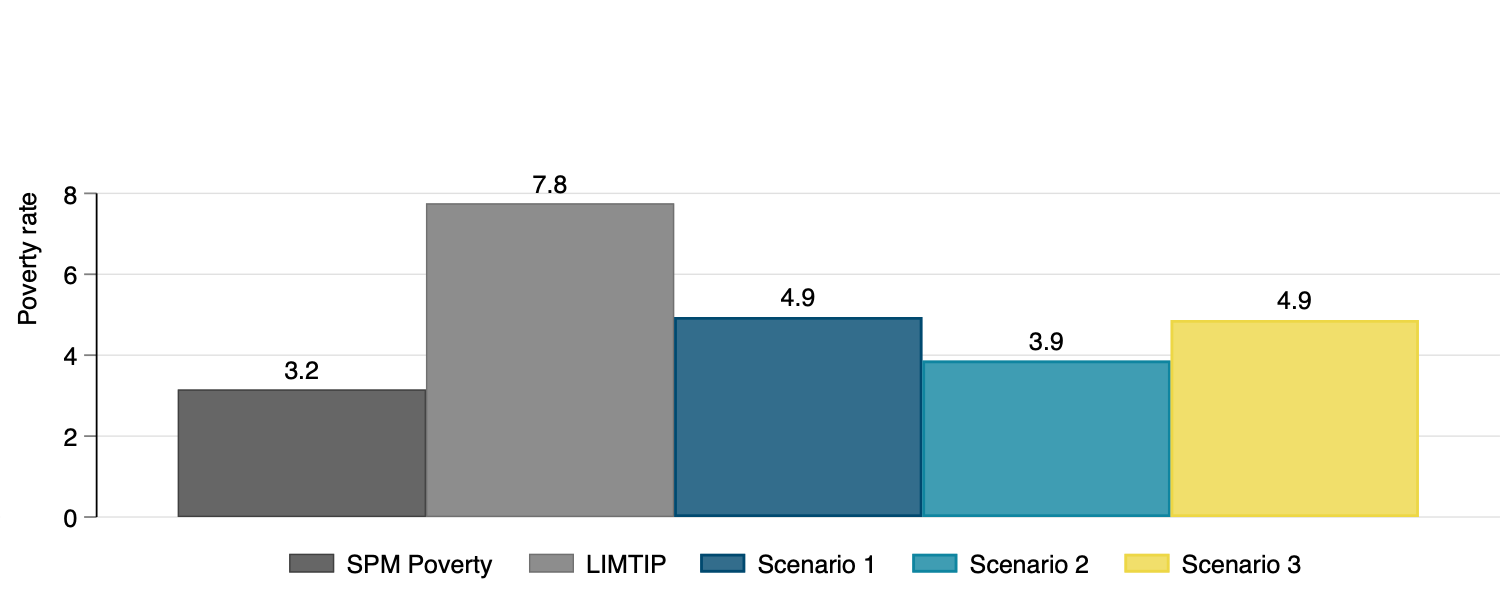
\includegraphics{../resources_brief/hh_pov_couple_brief2_all.png}

}

\caption{\label{fig-limtip}Changes in Poverty estimates across
redistribution scenarios}

\end{figure}%

Because there are many household members that could potentially take on
more household production responsibilities, the potential for
redistribution is high. However, the effectiveness depends considerably
on characteristics of the household, such as the presence of children,
the presence of other members, and the employment status of the wife.
Furthermore, because the redistribution scenarios are based on a
zero-sum game, there are individuals that may not benefit from
redistribution.

\begin{table}

\caption{\label{tbl-tb2}Time Poverty and Transition Rates}

\centering{

\begin{tabular}{l*{8}{c}cccccccccccccccc}
\hline\hline
          & \multicolumn{4}{c}{Men} & \multicolumn{4}{c}{Women} \\ 
\cline{2-5} \cline{6-9}
&          BL&         S.1&         S.2&        S. 3&          BL&         S.1&         S.2&        S. 3\\
\hline
All         &        44.2&        39.0&        24.2&        26.4&        61.4&        18.9&        22.5&        31.8\\
BL: Time NP &         0.0&        23.6&        19.7&        13.9&         0.0&         6.8&        15.9&        16.7\\
BL: Time P  &       100.0&        58.6&        29.8&        42.2&       100.0&        26.5&        26.6&        41.4\\
Household Type&           .&           .&           .&           .&           .&           .&           .&           .\\
\ All Mem. TP &       100.0&        95.8&        98.3&        82.4&       100.0&        68.7&        97.4&        81.8\\
\ At Least 1 Mem.time NP&        40.1&        82.5&        82.9&        55.8&        61.0&        53.6&        80.7&        65.2\\
\ Hhld can exit TP&        41.3&        24.1&         4.1&        15.1&        58.9&         6.6&         2.5&        19.9\\

\hline\hline
\end{tabular}

\footnotesize Note: BL refers to the baseline estimates

}

\end{table}%

In terms of incidence of time poverty, see Table~\ref{tbl-tb2}, women
benefit more from redistribution than men, except under Scenario 3. This
shows that even the simplistic redistribution rules we defined, the
gender wage gap has important implications in terms of women's time
poverty. The simulations also suggest that Scenario 2 is the most
effective in reducing time poverty for both men and women, bringing the
share of time poor individuals to 26.4\% (men) and 22.5\%(women).

These improvements do not come without casualties. Among non-time poor
men (baseline), we estimate that about 23\% of them could enter time
poverty under redistribution scenario 1, with a lower end of 13.9\%
under scenario 3. In contrast, while there is generally a smaller rate
of women falling into time poverty , the transition into poverty rate
under scenario 3 (16.7\%) is higher than that observed for men. This
reinforces the idea that gaps in opportunity costs/bargaining power can
have important implications for the redistribution of time and could
affect time poverty.

The type of the household also plays an important role in the
effectiveness of redistribution. Even in cases where everyone in the
household is time poor, redistribution can still reduce the time poverty
status of individuals. While this improvements are small for men, there
are significant reductions in time poverty for women under the equal
shares scenarios (Scenario 1). As we will see later, however, this
should not be interpreted as a general improvement, as someone else in
the household will have to take on the extra responsibilities, and thus
increasing their own and the household time decifit. The results that
appear to be the most paradoxical relate to households where there are
non-time poor individuals, but the total time surplus is not enough to
eliminate time poverty. In these households, based on individual time
poverty alone, it may seem that all redistribution scenarios have a
negative impact on both husbands and wives. However, despite the higher
time poverty incidence, there is also a reduction in time deficits that
should still improve overall welfare of the household.

Lastly, for household that can exit time poverty, most of their members
(husband and wife) will exit time poverty. And just as described before,
both men and women benefit greatly under Scenario 2, with scenario 1
being the least favorable for men, and scenario 3 the least favorable
for women.

\textbf{The role of household Structure}

The results we just presented provides us with an overall picture of the
potential of redistribution to reduce time poverty. However, the
effectiveness of redistribution also depends on the structure of the
household. There are two factors, as observed in Table~\ref{tbl-tb3},
that are important to understand how effective redistribution can be:
the presence of young children and the presence of other members in the
household.

On the one hand, presence of young children (14 years or younger) will
have a large impact on the requirements of household production, mostly
in the form of child care activities, without the possibility of the
children taking on any of the responsibilities.\footnote{By
  construction, the ATUS does not collect information on time use of
  individuals younger than 15} On the other hand, if there are other
members in the household, the potential for redistribution is higher, as
these members could potentially take on some of the responsibilities of
the couple.

Interestingly, at baseline, the presence of children, and presence of
other household members, are weakly associated with time poverty
differences across husband and wife. The small differences we observe
are as expected, with somewhat higher levels of time poverty across
households with children, and households without other members.

\begin{table}

\caption{\label{tbl-tb3}Time Poverty by Household Structure}

\centering{

\begin{tabular}{l*{8}{c}cccccccccccccccc}
\hline\hline
          & \multicolumn{4}{c}{Men} & \multicolumn{4}{c}{Women} \\  \cline{2-5} \cline{6-9}
            &    BL&  S. 1&  S. 2&  S. 3&    BL&  S. 1&  S. 2&  S. 3\\
Yng Children Presence & \multicolumn{8}{c}{} \\ 
\ \ No Children&          43.3&        24.3&        13.1&        17.1&        59.2&        11.5&        11.5&        19.7\\
\ With Children&        44.9&        50.9&        33.1&        33.9&        63.2&        24.8&        31.3&        41.6\\
\midrule

Other Members in HH    & \multicolumn{8}{c}{} \\ 
\ \ No      &        44.7&        44.1&        29.7&        32.0&        62.3&        22.1&        27.8&        39.4\\
\ Yes       &        42.5&        23.9&         7.6&         9.6&        58.7&         9.2&         6.4&         9.3\\
\hline\hline
\end{tabular}

\footnotesize Note: BL refers to the baseline estimates and S1, S2 and
S3 refer to the three scenarios respectively.

}

\end{table}%

When considering the impact of the redistribution scenarios, we find a
clear pattern that the presence of children and absence of other members
have a very similar impact reducing the effectiveness of redistribution
scenarios. In both cases, the reduction in time poverty we estimate for
women is still larger than that for men. This highlights how much more
work women do in taking care of the household, specially providing
primary child are, as well as absorbing most of the responsibilities of
the household production, when there are no other members to share the
responsabilities. This also explains why, when redistribution is
applied, the reduction in time poverty is more limited for husbands.

\textbf{Income and Employment}

One last aspect to consider is to analyze if there is any heterogeneity
in the estimated impact of redistribution based on the household overall
income or the employment status of the wife. We do not consider the
employment status of the husband, because 97.2\% of husbands are
employed, and thus, there is little variation to analyze. We should also
remember that we concentrate on households that are time poor, and thus
are less likely to be income poor, because one or both of the partners
are employed.

\begin{table}

\caption{\label{tbl-tb4}Time Poverty by Income}

\centering{

\begin{tabular}{l*{8}{c}cccccccccccccccc}
\hline\hline
          & \multicolumn{4}{c}{Men} & \multicolumn{4}{c}{Women} \\  \cline{2-5} \cline{6-9}
            &    BL&  S. 1&  S. 2&  S. 3&    BL&  S. 1&  S. 2&  S. 3\\
Income/Pline   & \multicolumn{8}{c}{} \\ 
\ \ < PLine &        45.0&        35.7&        12.2&        24.5&        56.6&        10.9&        11.3&        20.8\\
\ 1-2 x Pline&        42.5&        39.9&        20.2&        25.8&        60.3&        17.1&        18.0&        28.9\\
\ 2-4 x Pline&        43.3&        38.7&        25.1&        26.4&        62.3&        19.0&        23.4&        31.5\\
\ > 4 x Pline&        46.1&        39.3&        26.2&        27.0&        61.5&        20.4&        24.8&        34.9\\

\midrule

Wife Work Status   & \multicolumn{8}{c}{} \\ 
\ \ Not Working&        85.5&        67.7&         8.9&        50.2&        10.2&         0.0&         2.5&         0.1\\
\ Working   &           40.3&        36.4&        25.6&        24.2&        66.2&        20.6&        24.3&        34.8\\
\hline\hline
\end{tabular}

\footnotesize Note: BL refers to the baseline estimates and S1, S2 and
S3 refer to the three scenarios respectively.

}

\end{table}%

We first consider the impact of redistribution based on the household
income, or more specifically, the income-to-poverty-line ratio.
Interestingly, it may seem that time poverty, at baseline, does not
discriminate across income groups, showing similar levels across the
income distribution. Although we do observe a slightly lower share of
time poor women (56.6\%) in the lowest income group, compared to average
of 61.0\%.

For men, there is very little variation in the impact of redistribution
across income groups for scenarios 1 and 3. It may seem that men will
either increase their share of household production (Scenario 1) or will
take advantage of the opportunity cost of time (Scenario 3), regardless
of the income. For Scenario 2, however, we observe that redistribution
is more effective in reducing time poverty for those in the lowest
income group.

What is more interesting is that the same pattern of decreasing
effectiveness of redistribution policies is also observed among women,
for all scenarios. A possible explanation is that the share of employed
men does not vary much across income groups. However, the share of
non-employed women goes from about 30\% in the lowest income group, to
5\% in the highest income group. This means that for people in the
highest income group, there is less room for redistribution because both
husband and wife are employed. However, because women still take on most
of the household production, the impact of redistribution is still
higher for them compared to men.

\textbf{What about the Hidden Poor?}

One of the main contributions of the LIMTIP is the identification of the
hidden poor, i.e., individuals who are not classified as poor based on
official poverty estimates but are classified as such when one accounts
for the time deficits they face. In Table~\ref{tbl-tb5} we present the
hidden poor estimates by sub-groups. For our sample, we estimate that
4.6\% of the population which is not classified as officially poor, fall
under this definition when we adjust time deficits. However, if any of
the redistribution scenarios were to be implemented, the share of hidden
poor could be reduced to 0.7-1.8\%.

When considering household characteristics, redistribution scenarios
could actually increase hidden poverty in households where everyone is
time poor, but can be greatly reduced whenever there is room for
redistribution. For example, if the household has the potential to exit
time poverty, redistribution based on the time available principle could
almost eliminate the share of hidden poor (0.1\%).

Lastly, when the wife is working, redistribution based on equal shares
or opportunity cost are almost ineffective in reducing the share of
hidden poor, probably because the wife is already doing the bulk of
household production, and redistribution would only increase the time
poverty of other members. However, if she is working, as is the case for
91\% of the sample, redistribution will help reduce the double burden of
time women face.

\begin{table}

\caption{\label{tbl-tb5}Hidden Poor by Characteristics}

\centering{

\begin{tabular}{l*{4}{c}cccccccc}
\hline\hline
            &    Baseline&  Scenario 1&  Scenario 2&  Scenario 3\\
\hline
All         &           4.6&         1.8&         0.7&         1.7\\
\midrule

Household Type      & \multicolumn{4}{c}{} \\ 
\ \ All Mem. TP         &         5.2&         5.8&         5.6&         5.7\\
\ At Least 1 Mem.time NP&         6.8&         3.2&         1.8&         3.3\\
\ Hhld can exit TP&               4.0&         1.2&         0.1&         1.0\\

\midrule

Yng Children Presence & \multicolumn{4}{c}{} \\ 
\ \ No Children &         2.4&         0.7&         0.2&         0.7\\
\ With Children&         6.3&         2.7&         1.1&         2.5\\
\midrule

Other Members in HH      & \multicolumn{4}{c}{} \\ 
\ \ No      &         4.4&         2.0&         0.9&         2.0\\
\ Yes       &         5.3&         1.1&         0.2&         0.8\\

\midrule

Income/Pline     & \multicolumn{4}{c}{} \\ 
\ \ 1-2 x Pline&         23.1&         8.8&         3.4&         8.4\\
\ 2-4 x Pline&           0.3&          0.2&         0.2&         0.2\\

\midrule

Wife Work Status  & \multicolumn{4}{c}{} \\ 
\ \ Not Working         7.1&         7.0&         0.5&         4.7\\
\ Not working&          4.4&         1.3&         0.7&         1.4\\

\hline\hline
\end{tabular}

}

\end{table}%

\section{Policy Implications: Opportunities and
Challenges}\label{policy-implications-opportunities-and-challenges}

The findings in this policy brief suggest that intra-household
redistribution of household production is a potentially effective tool
to reduce time deficits and alleviate time poverty for individuals and
households. Our findings show that such redistributions can have
significant well-being effects, promoting more equitable sharing of
household responsibilities between husbands and wives and, in some
cases, lifting entire households out of poverty. Among the three
redistribution scenarios considered, the equity-based approach emerged
as the most effective in reducing poverty rates and enabling individuals
to exit poverty.

However, the effectiveness of redistribution policies is contingent on
the type and structure of households. For instance, in households where
all members are time-poor, redistribution may not be effective and could
potentially (slightly) increase LIMTIP poverty.

In contrast, households with sufficient time surpluses to absorb time
deficits can effectively eliminate time poverty under any of the
proposed redistribution policies. Moreover, presence of chilren in
housheodls demand more work and couples experience greater time poverty.
It is widely established in the literature presence of children impose
labor market particpation constraints, particularly among women
(Department, 2024).

While redistribution policy may be difficult to implement, public
polices can help target inequalities in terms of ``time availability''
and ``opportunity cost'' experienced by men and women, which are a
result of gender discriminatory vicious cycle that hinders equal
educational opportunities for women leading to unequal occupation
opportunities as well as earning cabailities (Sinha and Sedai (2024)).
Policy initiatives that can contribute towards a more gender-equitable
sharing of hosuehold production can be segregated into three broad
categories:

\begin{itemize}
\tightlist
\item
  Labor market or employment policies to reduce gender disparity: This
  would involve targetting equal pay at work for men and women and
  ensuring elimination of gender discrimination at workplace. Moreover,
  long-working hours that directly impact time constraints may also need
  to be regulated.
\item
  Public investment in care infrastructure and services: This can be
  helpful as it can contribute toward reducing the required hours of
  household production that determine people's time deficits and time
  poverty. In particular for married couples and those with childre,
  efforts can involve quality childcare services at subsidized rates and
  can even be even extended to a universal and centralized provisioning
  of care services. In addition, parental leave laws offering not only
  maternity leave benefits but those combined with paternity leaves may
  serve to have more gender-equitable effects on household division of
  labor.
\item
  Targeting social norms: Gender disparity in labor market are guided by
  gender norms defining gender roles. Targeting norms could involve
  educational interventions during early schooling years, gender
  equitable knowledge-sharing as part of couple counseling on how gender
  norms can be detrimental for the overall well-being and deevlopment of
  the society and the economy.
\end{itemize}

\section{Conclusion/recommendations}\label{conclusionrecommendations}

This policy brief has examined the potential of redistributing household
production responsibilities to alleviate time poverty in the United
States for married couples. Using the Levy Institute Measure of Time and
Income Poverty (LIMTIP), we have shown that time poverty is a
significant issue affecting married couples, such that about 48\% of
households with couples experience time poverty.

Our analysis of three redistribution scenarios - based on equality,
equity, and opportunity cost principles - reveals that such
redistributions can significantly reduce time poverty, particularly in
households where time surpluses exceed time deficits.

These findings underscore the importance of integrating time poverty in
poverty alleviation inititaives. They also highlight the potential of
intra-household redistribution as a policy tool to promote gender
equality and improve overall household well-being. However, the varying
effects across household types, household structures, poverty groups and
employment status of wives, along with variations across redistribution
scenarios suggest that a one-size-fits-all approach may not be optimal
and a targeted tailored approach is needed.

In conclusion, while redistribution of household production is promising
in alleviating time poverty, and the hidden poor, it should be
considered as part of strategies that also addresses societal and
structural factors affecting to time and income poverty.

\section*{References}\label{references}
\addcontentsline{toc}{section}{References}

\phantomsection\label{refs}
\begin{CSLReferences}{1}{0}
\bibitem[\citeproctext]{ref-addati2018}
Addati, L., Cattaneo, U., Esquivel, V., and Valarino, I. (2018).
\emph{Care work and care jobs for the future of decent work}.
International Labour Organisation (ILO).

\bibitem[\citeproctext]{ref-Antonopoulos2017}
Antonopoulos, R., Esquivel, V., Masterson, T., and Zacharias, A. (2017).
Time and income poverty in the city of buenos aires. In R. Connelly and
E. Kongar (Eds.), \emph{Gender and time use in a global context: The
economics of employment and unpaid labor} (pp. 161--192). Palgrave
Macmillan US. \url{https://doi.org/10.1057/978-1-137-56837-3_7}

\bibitem[\citeproctext]{ref-berik2009}
Berik, G., Rodgers, Y. van der M., and Seguino, S. (2009). Feminist
{Economics} of {Inequality}, {Development}, and {Growth}. \emph{Feminist
Economics}, \emph{15}(3), 1--33.
\url{https://ezprox.bard.edu/login?url=https://search.ebscohost.com/login.aspx?direct=true&db=ecn&AN=1063369&site=eds-live&scope=site}

\bibitem[\citeproctext]{ref-hundt1996}
Bruyn-Hundt, M. (1996). Scenarios for a redistribution of unpaid work in
the netherlands. \emph{Feminist Economics}, \emph{2}(3), 129--133.
\url{https://doi.org/10.1080/13545709610001707826}

\bibitem[\citeproctext]{ref-ILO2024}
Department, I. L. Organization. S. (2024). \emph{The impact of care
responsibilities on women's labour force participation}. ILO.
\url{https://doi.org/10.54394/LPTT5569}

\bibitem[\citeproctext]{ref-duflo2012}
Duflo, E. (2012). Women {Empowerment} and {Economic} {Development}.
\emph{Journal of Economic Literature}, \emph{50}(4), 1051--1079.
\url{https://doi.org/10.1257/jel.50.4.1051}

\bibitem[\citeproctext]{ref-elson2017}
Elso, D. (2017). \emph{Recognize, {Reduce}, and {Redistribute} {Unpaid}
{Care} {Work}: {How} to {Close} the {Gender} {Gap}}.
\url{https://doi.org/10.1177/1095796017700135}

\bibitem[\citeproctext]{ref-elson2009}
Elson, D. (2009). Gender {Equality} and {Economic} {Growth} in the
{World} {Bank} {World} {Development} {Report} 2006. \emph{Feminist
Economics}, \emph{15}(3), 35--59.
\url{https://doi.org/10.1080/13545700902964303}

\bibitem[\citeproctext]{ref-valeria2016}
Esquivel, V. (2016). Power and the {Sustainable} {Development} {Goals}:
A feminist analysis. \emph{Gender \& Development}, \emph{24}(1), 9--23.
\url{https://doi.org/10.1080/13552074.2016.1147872}

\bibitem[\citeproctext]{ref-heckman1979}
Heckman, J. J. (1979). Sample selection bias as a specification error.
\emph{Econometrica}, \emph{47}(1), 153.
\url{https://doi.org/10.2307/1912352}

\bibitem[\citeproctext]{ref-hess2020}
Hess, Cynthia, Ahmed, T., and Hayes, J. (2020). \emph{Providing {Unpaid}
{Household} and {Care} {Work} in the {United} {States}: {Uncovering}
{Inequality}}.

\bibitem[\citeproctext]{ref-malik2018}
Malik, R., Hamm, K., Schochet, L., Novoa, C., Workman, S., and
Jessen-Howard, S. (2018). America's {Child} {Care} {Deserts} in 2018.
\emph{Center for American Progress}.
\url{https://www.americanprogress.org/article/americas-child-care-deserts-2018/}

\bibitem[\citeproctext]{ref-masterson2012}
Masterson, T. (2012). \emph{Simulations of full-time employment and
household work in the levy institute measure of time and income poverty
(LIMTIP) for argentina, chile, and mexico} (Working Paper 727; Levy
Economics Institute Working Paper). Levy Economics Institute of Bard
College.

\bibitem[\citeproctext]{ref-masterspm2022}
Masterson, T., Antonopoulos, R., Nassif-Pires, L., Rios-Avila, F., and
Zacharias, A. (2022). \emph{Assessing the impact of childcare expansion
in mexico: Time use, employment, and poverty} {[}Research Project
Report{]}. Levy Economics Institute of Bard College.
\url{https://www.levyinstitute.org/pubs/rpr_6_22.pdf}

\bibitem[\citeproctext]{ref-oecd2020}
OECD. (2020). \emph{Early learning and child well-being in the united
states} (p. 124).
https://doi.org/\url{https://doi.org/https://doi.org/10.1787/198d8c99-en}

\bibitem[\citeproctext]{ref-rein2023}
Reinhard, S. C., Caldera, S., Houser, A., and Choula, R. (2023).
\emph{Valuing the {Invaluable}: 2023 {Update}}. AARP Public Policy
Institute. \url{https://doi.org/10.26419/ppi.00082.006}

\bibitem[\citeproctext]{ref-sinha2024}
Sinha, A., and Sedai, A. K. (2024). Why {Care} for the {Care} {Economy}:
{Empirical} {Evidence} from {Nepal}. \emph{Eastern Economic Journal},
\emph{50}(3), 337--373. \url{https://doi.org/10.1057/s41302-024-00282-5}

\bibitem[\citeproctext]{ref-zacharias2011}
Zacharias, A. (2011). \emph{The measurement of time and income poverty}
(Working Paper 690; Levy Economics Institute Working Paper). Levy
Economics Institute of Bard College.

\bibitem[\citeproctext]{ref-zacharias2012}
Zacharias, A., Antonopoulos, R., and Masterson, T. (2012). \emph{Why
time deficits matter: Implications for the measurement of poverty}
{[}Research Project Report{]}. Levy Economics Institute of Bard College.
\url{https://www.levyinstitute.org/pubs/rpr_08_12}

\bibitem[\citeproctext]{ref-zacharias2014}
Zacharias, A., Masterson, T., and Kim, K. (2014). \emph{The measurement
of time and income poverty in korea: The levy institute measure of time
and income poverty} {[}Research Project Report{]}. Levy Economics
Institute of Bard College.
\url{https://www.levyinstitute.org/pubs/rpr_8_14}

\bibitem[\citeproctext]{ref-zacharias2018}
Zacharias, A., Masterson, T., Rios-Avila, F., Kim, K., and
Khitarishvili, T. (2018). \emph{The measurement of time and income
poverty in ghana and tanzania: The levy institute measure of time and
consumption poverty} {[}Research Project Report{]}. Levy Economics
Institute of Bard College.
\url{https://www.levyinstitute.org/pubs/rpr_8_18}

\bibitem[\citeproctext]{ref-zacharias2021}
Zacharias, A., Masterson, T., Rios-Avila, F., and Oduro, A. D. (2021).
\emph{Scope and effects of reducing time deficits via intrahousehold
redistribution of household production: Evidence from sub-saharan
africa: The levy institute measure of time and consumption poverty}
{[}Research Project Report{]}. Levy Economics Institute of Bard
College.\href{\%20https://www.levyinstitute.org/pubs/rpr_7_21.pdf}{https://www.levyinstitute.org/pubs/rpr\_7\_21.pdf}

\bibitem[\citeproctext]{ref-zacharias2024a}
Zacharias, A., Rios-Avila, F., Folbre, N., and Masterson, T. (2024).
\emph{Integrating nonmarket consumption into the bureau of labor
statistics consumer expenditure survey} {[}Research Project Report{]}.
Levy Economics Institute of Bard
College.\href{\%20https://www.bls.gov/cex/consumption/integrating-nonmarket-consumption-bls-consumer-expenditure-survey.pdf}{https://www.bls.gov/cex/consumption/integrating-nonmarket-consumption-bls-consumer-expenditure-survey.pdf}

\end{CSLReferences}



\end{document}
